\documentclass[letterpaper]{article}

\usepackage{natbib,alifeconf}  %% The order is important
\usepackage{graphicx,booktabs,amsmath}
\usepackage[hyphens]{url}
\usepackage[hidelinks]{hyperref}

\newcommand{\cond}[1]{\texttt{#1}}

\title{What a Lineage Learns: Thirty-Nine Pre-registered Predictions\\in a Sealed Artificial World with a River}

\author{Lachlan Bremner \\
\mbox{}\\
Independent researcher, Perth, Western Australia \\
ORCID 0009-0007-8818-4607}

\begin{document}
\maketitle

\begin{abstract}
We report six experiments in \emph{river world}, a sealed artificial ecosystem in which tabular
Q-learning agents live inside an evolving population under a strictly conserved energy budget, on a
cylinder of land split by a river that can be crossed only at fords. Nine conditions were run for
sixteen seeds each, to 2,000 simulated years and, for four of them, to 10,000: 800,000
seed-years in all. Thirty-nine predictions were written down before the runs they concern and are
scored here unedited: 17 held, 5 held in part and 17 failed. Three results stand out. First, the
apparent Baldwin-style effect, evolution turning down the learning rate when learned values are not
inherited, is a transient: the ratio between arms peaks at 3.7 near year 300 and falls to 1.2 by year
10,000, so inheritance changes how fast the learning rate converges, not where. Second, inheriting
learned values is the only route to a signalling habit: a 0.05 energy cost to speak is invisible to
one lifetime of learning but is learned by a lineage, and 83\% of inheriting agents end up favouring
silence against 33\% without inheritance. Third, walling the river off entirely produces no divergence
in signalling between the banks, because the channel offers a cost gradient rather than an arbitrary
convention to diverge on. The failed predictions were the informative ones: each cluster of failures
pointed at a place where the model's mechanism differed from its description.
\end{abstract}

\section{Introduction}

Artificial life has long asked how learning within a lifetime and evolution across lifetimes shape
each other \citep{baldwin1896,hinton1987,ackley1991}, whether learned knowledge passed directly to
offspring helps or harms a population \citep{ackley1994}, and whether isolated populations of
communicating agents drift into distinct conventions \citep{steels1995,kirby2002}. Persistent
multi-agent worlds \citep{ray1991,yaeger1994,suarez2019} make these questions testable over long
horizons, and open-endedness gives them urgency \citep{bedau2000,packard2019,hughes2024}.

Recent work keeps these questions open. Direct inheritance of learned or epigenetic state is again
being compared with the Baldwin effect, in evolutionary computation \citep{benito2026} and on
compositional tasks, where it accelerates learning \citep{le2026}. Populations of learning agents
have been evolved in large worlds that are never reset \citep{hamon2023}, cultural knowledge has been
shown to accumulate across generations of reinforcement learners \citep{cook2024}, and novelty,
complexity and adaptation have been measured side by side in an open-ended system \citep{moreno2024}.
River world sits where these meet: learners inside an evolving, never-reset population, with the
inheritance rule as an experimental switch and a barrier that can isolate two halves of the culture.

These worlds also make it easy to tell a story afterwards. A long run produces dozens of time series,
and with enough of them some pattern can always be found and explained. Experimental psychology's
answer to the same problem is pre-registration: writing the prediction, and what would falsify it,
before the data exist \citep{nosek2018}. It is rare in artificial life.

This paper applies it to one world. We built river world to join a lifetime learner to an evolving
population under a fixed energy budget, wrote a set of predictions for six experiments, ran them,
and score every prediction here, including the seventeen that failed. Our contributions are:

\begin{itemize}
\setlength\itemsep{0pt}
\item A sealed, energy-conserving world combining tabular Q-learning, a heritable genome that tunes
  learning, and a geographic barrier, reproducible byte for byte across machines.
\item Evidence that the Baldwin-style divergence in learning rate between inheriting and
  non-inheriting populations is transient, and that its size depends on when it is measured.
\item A case of lineage-level learning: a behaviour too costly to show up within one life, acquired
  by a lineage through inherited value estimates.
\item A null result for isolation and signalling, explained by the shape of the signal channel's
  costs, with the experiment that would test the explanation.
\item A full scorecard of 39 pre-registered predictions, and what the failures revealed.
\end{itemize}

\section{The model}

\begin{figure}[t]
\centering
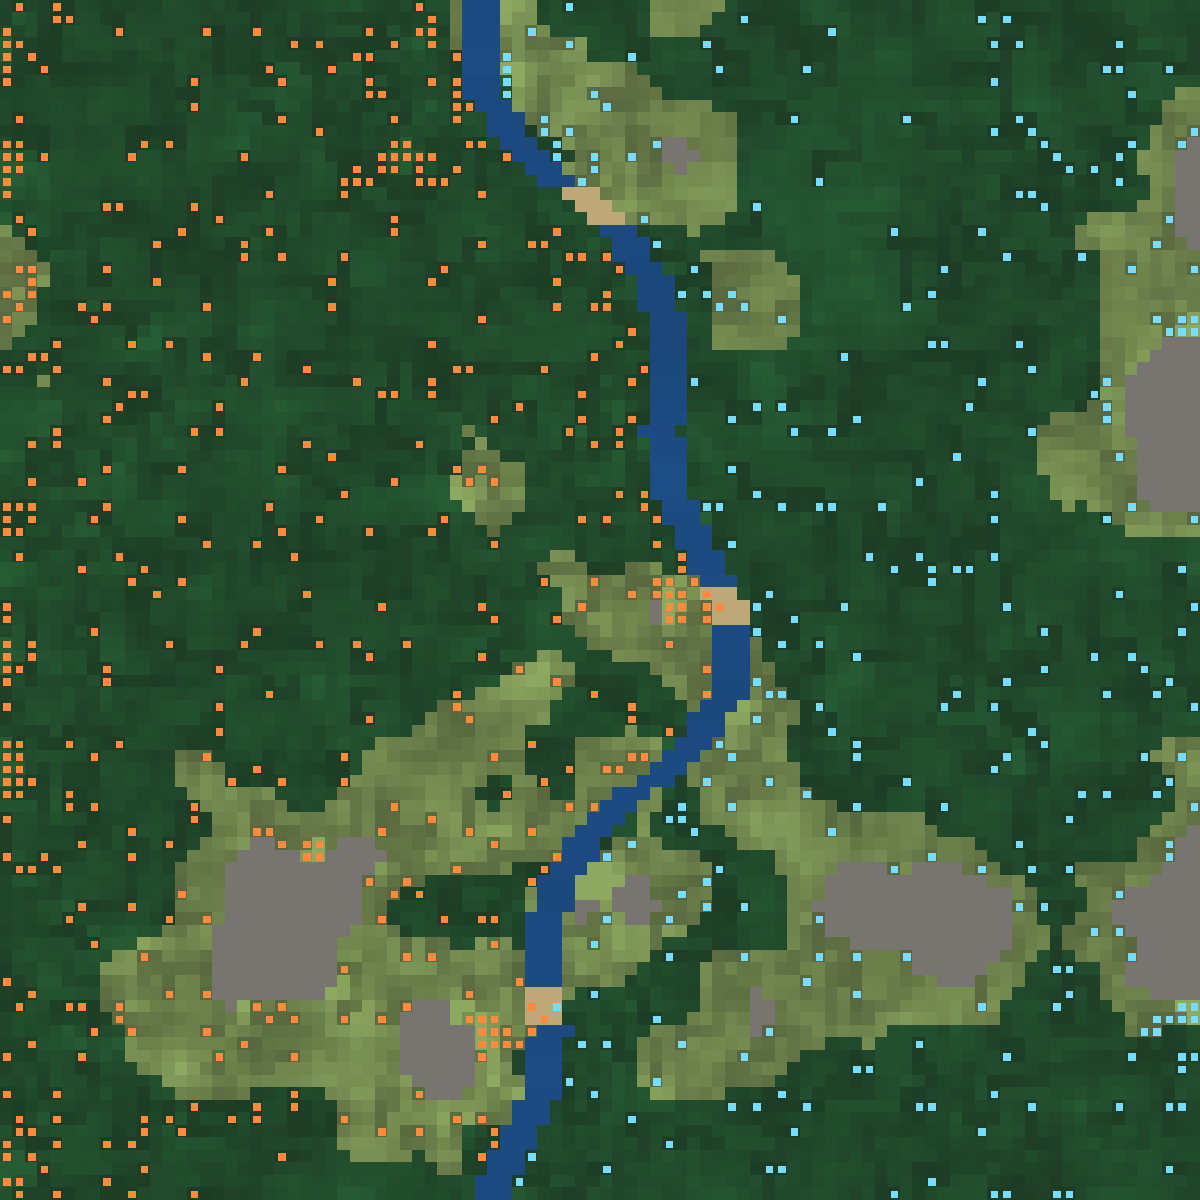
\includegraphics[width=\columnwidth]{figures/fig-river-map.pdf}
\caption{River world after 300 simulated years (one seed, learning inherited). The river runs north
to south and wraps round; tan bars are the three fords. Agents are coloured by bank. Paler land holds
more nutrients.}
\label{fig:map}
\end{figure}

\paragraph{World.} The world is a grid of $96 \times 96$ cells that wraps north to south and is walled
east to west, so it is a cylinder (Figure~\ref{fig:map}). Terrain is forest, clearings (22\% of cells)
and impassable rock (5\%). A river three cells wide meanders down the length of the cylinder and can be
crossed only at three fords. Time runs in ticks: a day is 20 ticks, the last 8 of them night, a season
100 and a year 400.

\paragraph{Energy.} The world holds 30,000 energy units, and none is ever created or destroyed; the
total is asserted after every tick. Energy sits in four pools: nutrients on the land, the river's
suspended load, agents' bodies and detritus. Agents eat nutrients (up to 4 a tick, at most 150 held)
and pay 0.5 a tick to rest and 0.9 to move, a quarter more at night. A dead agent becomes detritus,
which decomposes back into nutrients at 2 to 5\% a tick by terrain, faster in spring and slower in
winter. Nutrients diffuse 2\% a tick to each land neighbour. The river erodes 0.2\% of bank nutrients
a tick, carries its load downstream and deposits 1\% as silt. Seasonal events (spring floods, summer
droughts, fires of radius 6) change these rates but never the total (Figure~\ref{fig:energy}).

\begin{figure}[t]
\centering
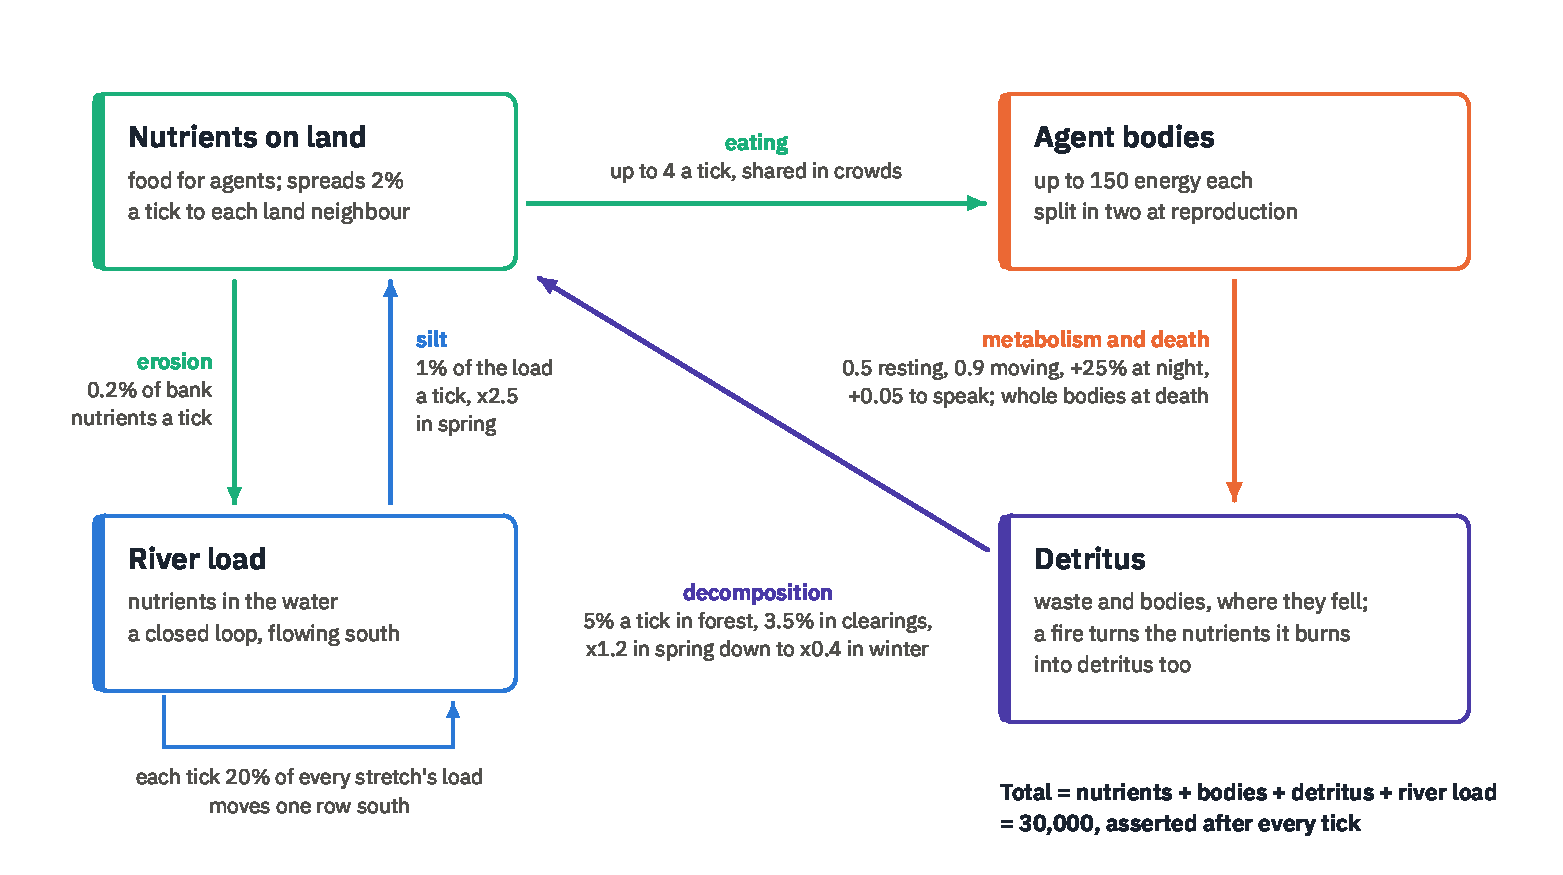
\includegraphics[width=\columnwidth]{figures/fig-energy-flow.pdf}
\caption{Where the energy goes. Four pools hold all 30,000 units; arrows are the only ways energy
moves between them. Events change the rates on the arrows, never the total.}
\label{fig:energy}
\end{figure}

\paragraph{Agents.} Each action pairs a move (stay or one of four directions) with a signal (silent
or one of three symbols), 20 actions in all. An agent hears the loudest signal in its eight
neighbouring cells one tick later; speaking costs 0.05 energy a tick, whichever symbol is used. Each
agent is a tabular Q-learner \citep{watkins1992} over 240 states: the direction of the richest
neighbouring cell, its energy band, day or night, the signal it hears and whether it is near water.
The reward is the change in its own energy; the discount is 0.95.

\paragraph{Evolution.} An agent with energy above a heritable threshold splits it with a child. The
genome has five genes: lifespan, the reproduction threshold, the mutation scale, the learning rate
$\alpha$ (starting at 0.2) and the exploration rate $\varepsilon$ (starting at 0.1). Evolution can
therefore tune the learning machinery itself: in \citet{hinton1987} the genome decides which traits
are left to learning, whereas here it sets the learning and exploration rates. What the child receives of its parent's
learning is set by a switch: \cond{copy} hands over the parent's Q-table (Lamarckian inheritance of
learned values), \cond{half} hands it over at half strength, and \cond{none} starts every child blank,
so only the genes for learning are inherited. The default is \cond{copy}.

\section{Method}

\begin{table}[t]
\centering
\footnotesize
\caption{The nine conditions. Anything not named is at the default: $96\times96$ cells, 30,000
energy units, a 2,000-agent cap, \cond{copy} inheritance, events on.}
\label{tab:conditions}
\begin{tabular}{@{}llll@{}}
\toprule
Condition & Change & Exp. & Years \\
\midrule
\cond{base}  & none                                 & all     & 10,000 \\
\cond{none}  & inherit none                         & E1, E2  & 10,000 \\
\cond{half}  & inherit half                         & E1, E2  & 2,000 \\
\cond{calm}  & no events                            & E4      & 2,000 \\
\cond{e20k}  & 20k energy                           & E5      & 2,000 \\
\cond{e45k}  & 45k energy, cap 3k                   & E5      & 2,000 \\
\cond{big}   & $128^2$, 53k energy, cap 3.5k        & E6      & 2,000 \\
\cond{ford1} & one ford                             & E3      & 10,000 \\
\cond{wall}  & no fords                             & E3      & 10,000 \\
\bottomrule
\end{tabular}
\end{table}

\paragraph{Experiments.} Six experiments each change one thing against the defaults
(Table~\ref{tab:conditions}). E1 and E2 ask whether learning should be inherited; E3 whether the river
is a barrier to culture; E4 whether disturbance keeps the world varied, after the intermediate
disturbance hypothesis \citep{connell1978}; E5 whether the population is limited by starvation or by
crowding; and E6 whether a bigger world sustains more variety. The agent cap sits at about twice the
expected population and is scaled with energy so that it never binds.

\paragraph{Runs.} Every condition ran sixteen seeds to year 2,000. Four conditions were carried on to
year 10,000, chosen by a trend test over years 1,500 to 2,000 rather than by taste: \cond{base} was
still moving, \cond{ford1} and \cond{wall} were E3's arms, and \cond{none} is the control for E2. That
is 800,000 seed-years, run on a single 16-core desktop at about 1.1 simulated years a second per
process. Every logged quantity is a per-year population statistic: population, the five gene means,
the number of states visited, policy complexity, lineage depth, signal entropy, the Jensen--Shannon
divergence between the two banks' signal distributions (\cond{dialect\_jsd}), crossings, the share of
the population on each bank and a behaviour-descriptor archive, from which a novelty count is derived in the spirit of the MODES
novelty metric \citep{dolson2019}.

\paragraph{Reproducibility.} A seed determines a world. Seeds 1 to 4 of \cond{base}, regenerated from
scratch on the desktop, reproduced a 300-year run of the same seeds made earlier on a laptop with a
different processor, on every one of 24 logged columns, byte for byte, except the floating-point
residue of the conservation check. A stopped run resumes exactly.
Energy drift stays near one part in $10^{12}$ of the total.

\paragraph{Pre-registration.} Twenty-six predictions, each with a number that would make it wrong,
were written to a dated file before the first world was created. Four more were added for \cond{e45k}
while it was still running, after \cond{e20k} had finished, and nine more before the four long runs
were carried past year 2,000. None has been edited; the file is archived with the data
\citep{bremner2026data}. Comparisons use Welch's $t$ over the last 100 years, sixteen seeds a side.
Because each comparison tests about twenty-two columns, we treat only $|t| > 4$ as a result.

\section{Results}

\subsection{Inheritance: a transient gap and a permanent habit}

\begin{figure*}[t]
\centering
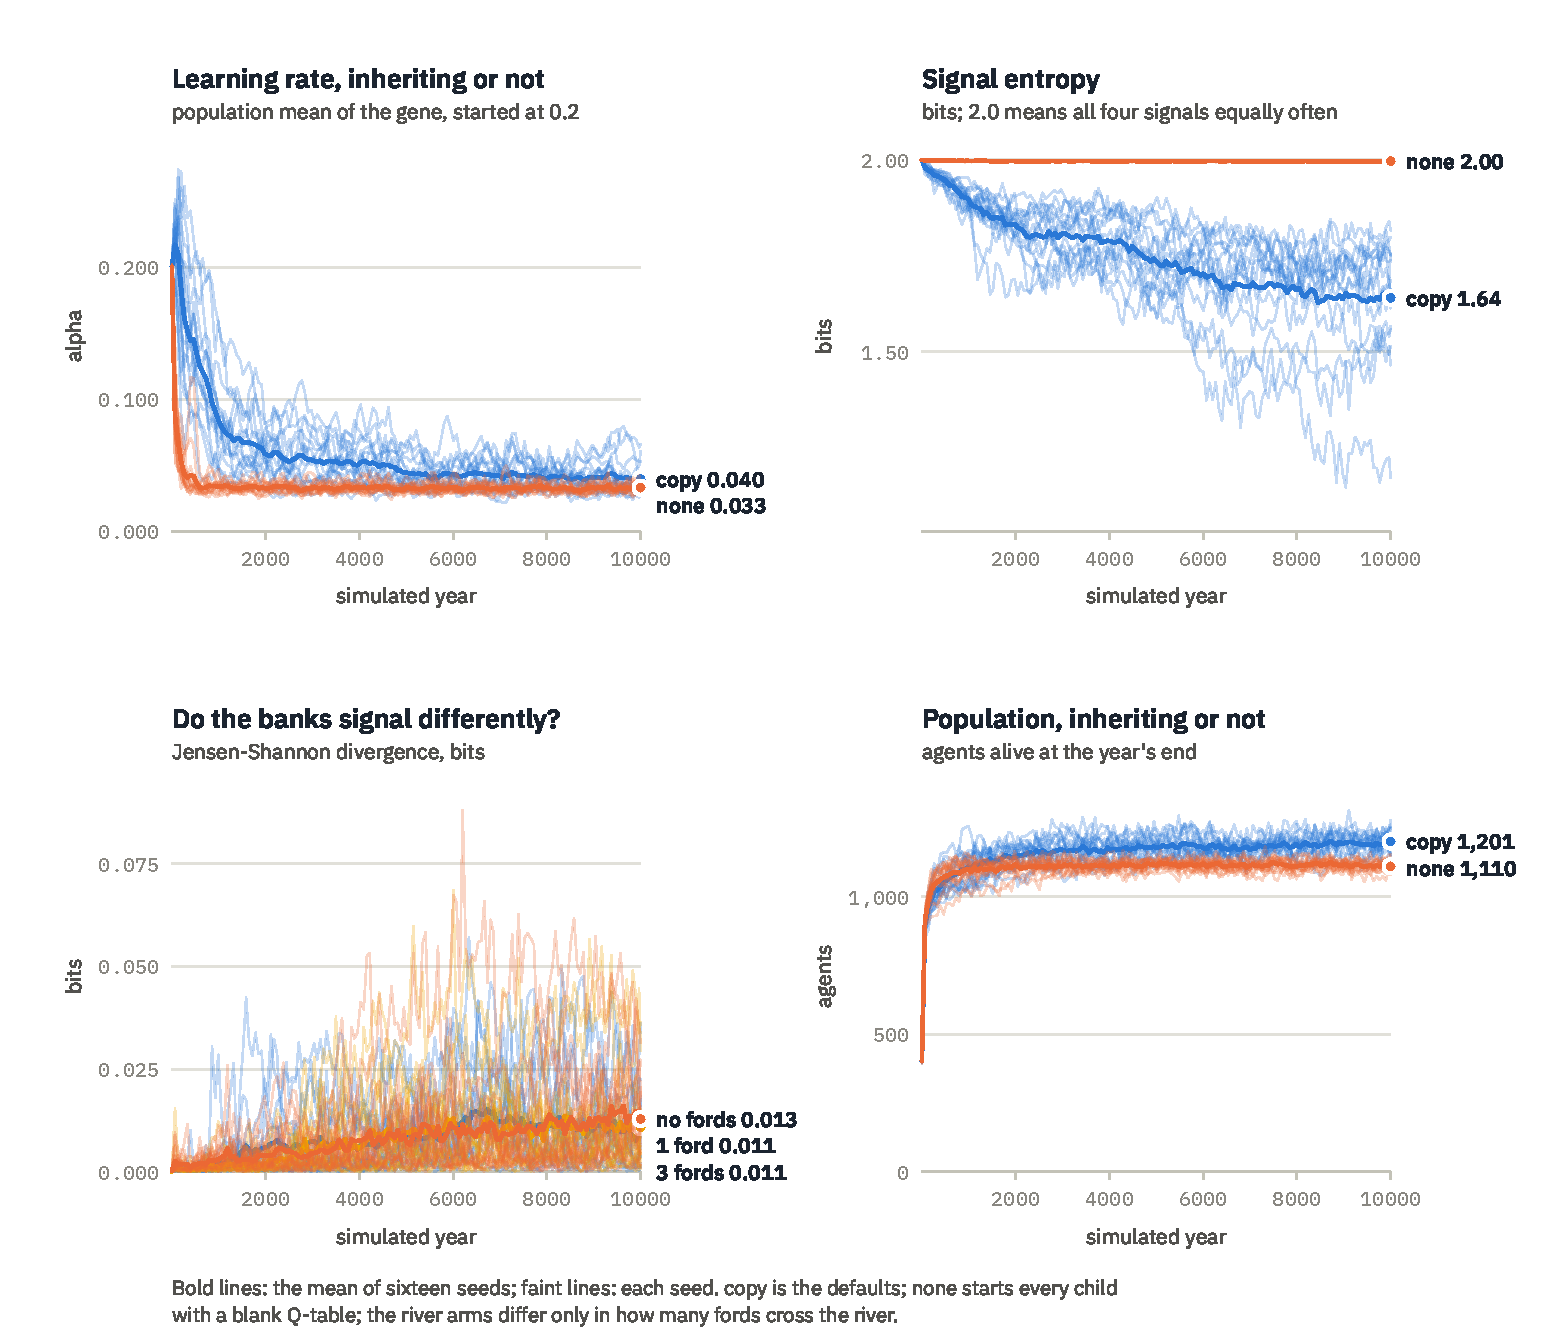
\includegraphics[width=0.82\textwidth]{figures/fig-s7-long.pdf}
\caption{The four conditions carried on to year 10,000, sixteen seeds each; bold lines are the mean,
faint lines individual seeds. Top left: the learning-rate gap between \cond{copy} (blue) and
\cond{none} (orange) closes to within seed noise. Top right: only the inheriting world structures its
signalling. Bottom left: the river arms stay together throughout. Bottom right: inheriting learned
values supports 8\% more agents, permanently.}
\label{fig:long}
\end{figure*}

\begin{figure*}[t]
\centering
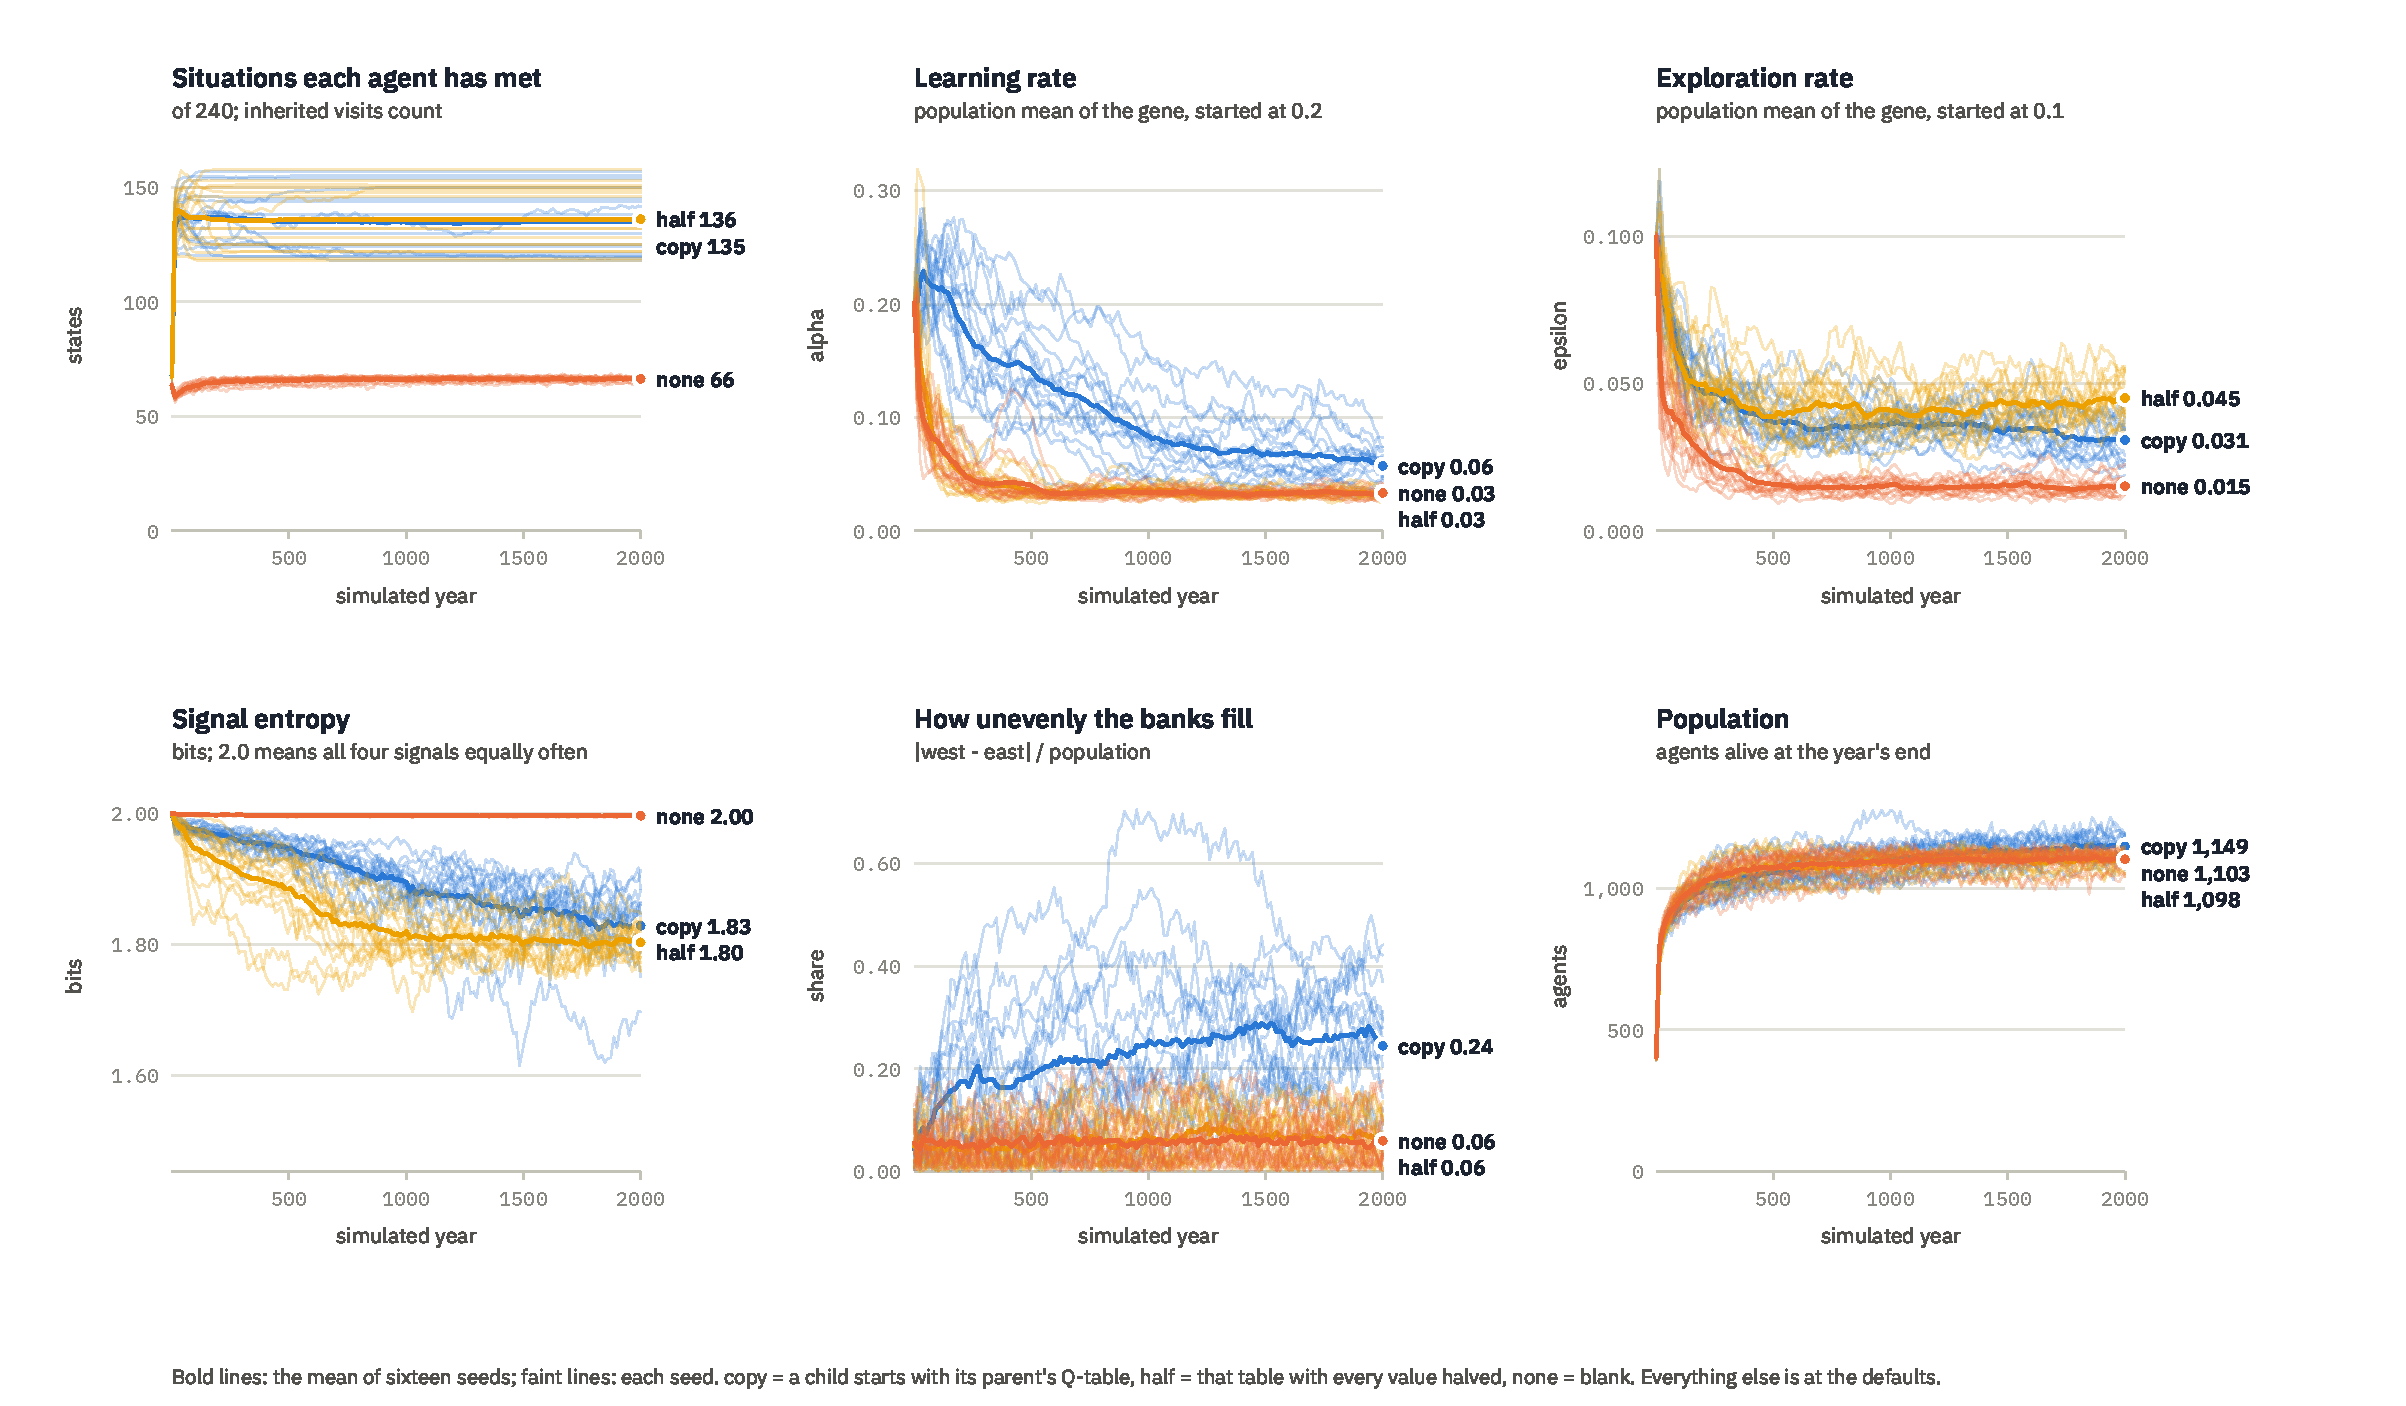
\includegraphics[width=0.92\textwidth]{figures/fig-s7-inherit.pdf}
\caption{Three inheritance rules over 2,000 years, sixteen seeds each; bold lines are the mean, faint
lines individual seeds. The learning-rate gap is real and narrowing, and the middle rule
(\cond{half}) does not produce a middle world.}
\label{fig:inherit}
\end{figure*}

\begin{table}[t]
\centering
\footnotesize
\caption{Mean learning-rate gene over the 100 years ending at each year shown, sixteen seeds an
arm. The ratio peaks near year 300 and decays.}
\label{tab:alpha}
\setlength\tabcolsep{3.2pt}
\begin{tabular}{@{}lrrrrrr@{}}
\toprule
Year & 100 & 300 & 1k & 2k & 5k & 10k \\
\midrule
\cond{copy} & 0.216 & 0.168 & 0.089 & 0.061 & 0.044 & 0.039 \\
\cond{none} & 0.108 & 0.045 & 0.034 & 0.033 & 0.032 & 0.033 \\
Ratio        & 2.0   & 3.7   & 2.6   & 1.86  & 1.37  & 1.20  \\
\bottomrule
\end{tabular}
\end{table}

\paragraph{The Baldwin gap is a transient.} When children start blank, evolution turns the learning
rate down quickly; when they inherit their parent's Q-table, it falls too, but later
(Figures~\ref{fig:inherit} and~\ref{fig:long}, Table~\ref{tab:alpha}). The ratio of the two arms' mean $\alpha$, as 100-year means, was 3.7 at year 300, 2.6 at 1,000,
1.86 at 2,000, 1.37 at 5,000 and 1.20 at 10,000, where $t = 2.3$. The \cond{none} arm reached
$\alpha \approx 0.034$ by year 1,000 and has stayed between 0.032 and 0.034 since. Read at year 300,
this would be a large, permanent effect of inheritance on learning; read at year 10,000, it is a
difference in how long the population takes to reach the same place. Exploration has narrowed less
(ratio 2.1 to 1.5) and still separates at $t = 5.7$.

\paragraph{A halfway rule is not a halfway world.} The \cond{half} arm was meant to land between the
other two. It does not: it matches \cond{copy} on states visited and \cond{none} on the learning-rate
gene, and on exploration it lies outside both. The cause is one line of code. A child receives the
parent's whole visited mask and every value halved, so the halving compounds down the generations.
Reading the checkpoints at year 2,000, a \cond{half} agent has visited as many states as a \cond{copy}
agent (136 of 240 against 135) but holds values 115 times weaker, weaker than what a blank agent
learns for itself in one life. Halving preserves which action is best but not how strongly it is
preferred, and evolution tunes the learning rate as though nothing were inherited.

\begin{table}[t]
\centering
\footnotesize
\caption{\cond{copy} against \cond{none} at year 10,000: means over years 9,901 to 10,000, sixteen
seeds a side.}
\label{tab:long}
\begin{tabular}{@{}lrrr@{}}
\toprule
Measure & \cond{copy} & \cond{none} & $t$ \\
\midrule
Learning rate $\alpha$       & 0.0391 & 0.0326 & 2.3 \\
Exploration $\varepsilon$    & 0.0212 & 0.0145 & 5.7 \\
Signal entropy (bits)        & 1.654  & 1.997  & $-8.9$ \\
Favourite signal is silence  & 83\%   & 33\%   & \\
Population                   & 1,198  & 1,111  & 9.8 \\
Generations deep             & 2,462  & 1,793  & 14.4 \\
Nutrients standing on land   & 4,839  & 4,155  & 15.2 \\
Crossings a year             & 183    & 318    & $-4.7$ \\
\bottomrule
\end{tabular}
\end{table}

\paragraph{A habit only a lineage can learn.} Without inheritance, signal entropy stays at 1.997 bits
of a possible 2.0 for all 10,000 years: the four signals are used almost exactly equally, and silence
is the favourite of 33\% of agents against the 25\% chance would give (Table~\ref{tab:long}). With
inheritance, silence is the favourite of 83\%. Speaking costs 0.05 energy a tick, a cost too small
for one lifetime of Q-learning to detect against the noise of feeding, and large enough to show once
the estimate is carried down 2,400 generations. This is a behaviour that no individual learns and a
lineage does.

\paragraph{Inherited learning feeds more agents.} The inheriting world holds 7.8\% more agents
($t = 9.8$), a gap present at every 1,000-year checkpoint from year 2,000. It also leaves more
nutrients standing and holds more energy in each body, so the extra agents come from grazing better
rather than harder. The blank world's standing crop has been flat at 4,153 to 4,155 units since year
2,000; the inheriting world's rose from 4,544 to 4,839 and was still rising when the run stopped.

\subsection{Isolation does not separate the banks}

\begin{figure}[t]
\centering
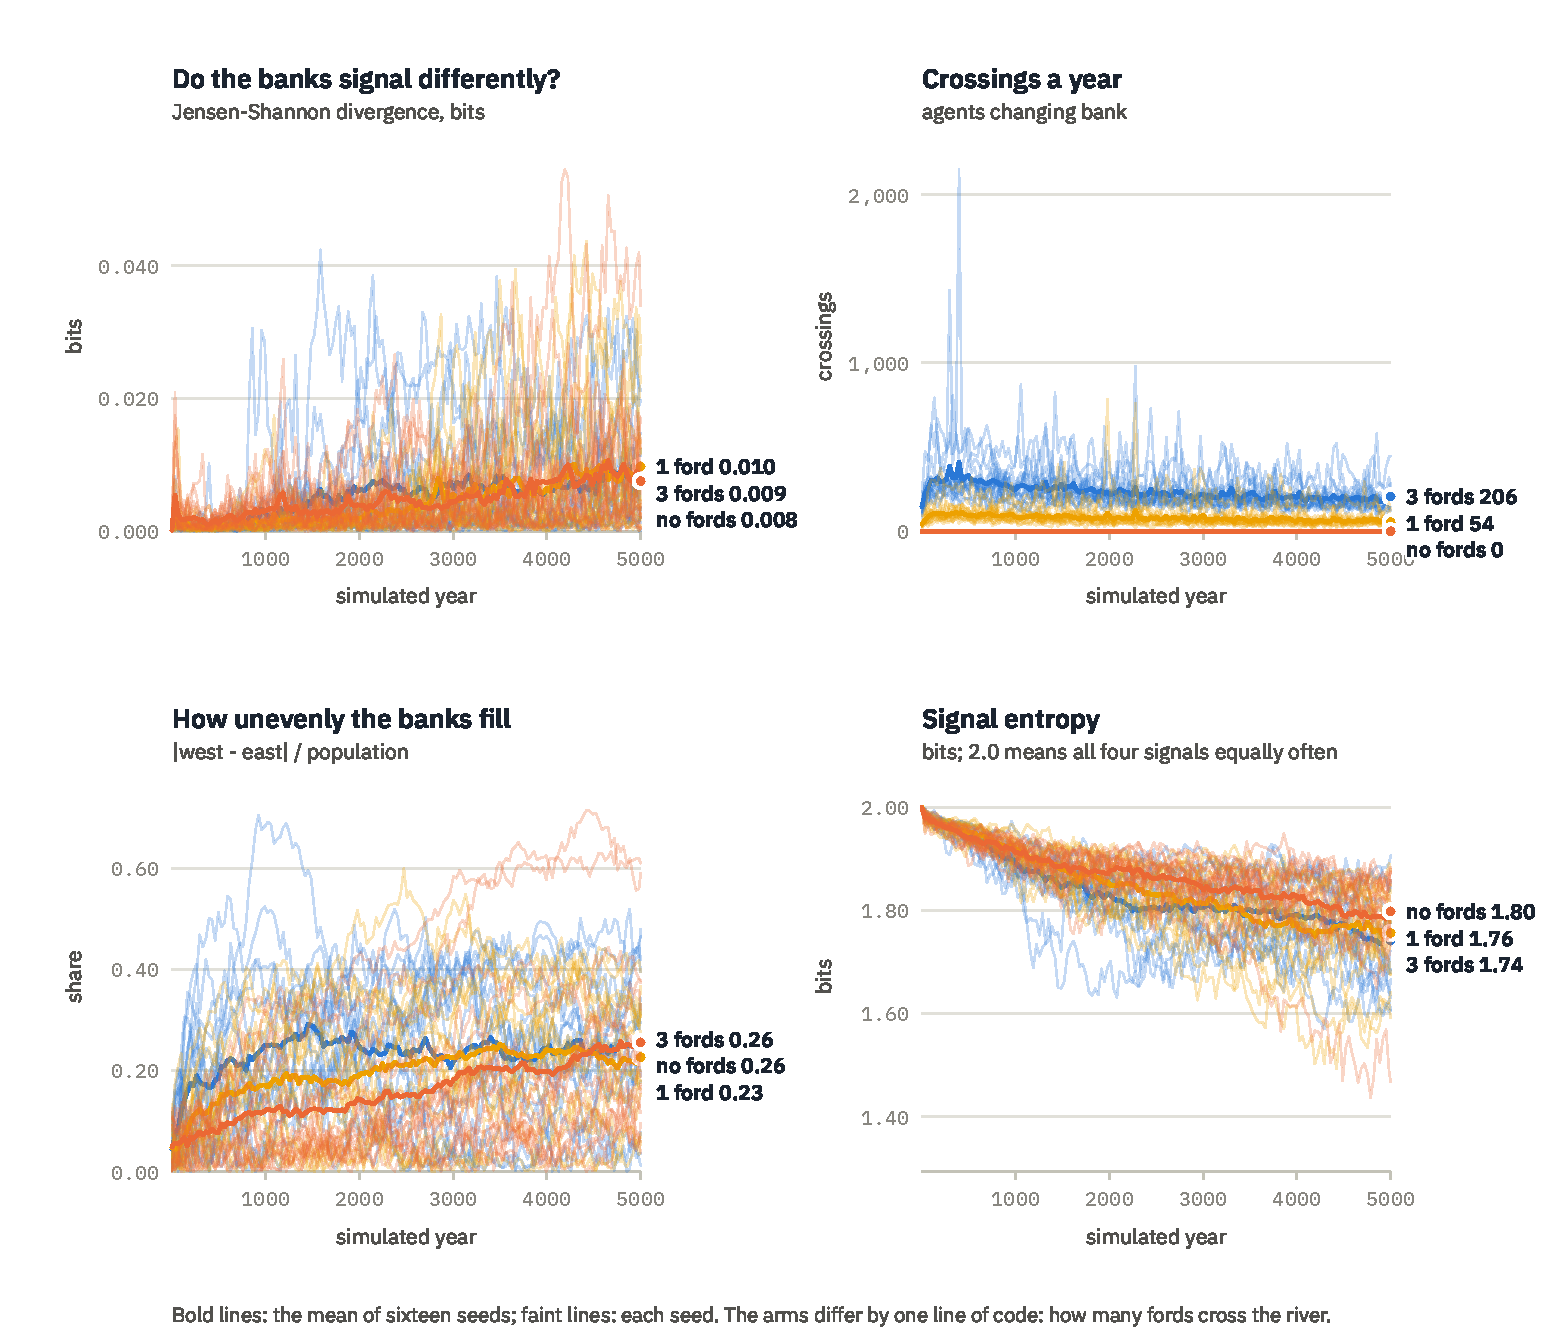
\includegraphics[width=\columnwidth]{figures/fig-s7-river.pdf}
\caption{E3, sixteen seeds an arm over 5,000 years. Crossings fall from about 200 a year (three
fords) to about 60 (one ford) to none (wall); the divergence between the banks' signalling does not
move with them.}
\label{fig:river}
\end{figure}

Walling the river completely cut crossings to zero in every one of \cond{wall}'s 80,000 seed-years
to year 5,000, and one ford cut them to a third. Nothing downstream followed (Figure~\ref{fig:river}).
At year 5,000, the pre-registered horizon, \cond{dialect\_jsd} was 0.0086 bits with three fords,
0.0090 with one and 0.0083 with none ($t = 0.12$, wall against three fords). All three arms drift
upward together, from about 0.001 at year 500, which is a property of the world ageing rather than of
its geography. At year 10,000 the values are 0.0098, 0.0100 and 0.0130 ($t = 0.98$). The largest
single seed-year in any arm in 10,000 years was 0.096; the pre-registered threshold for a dialect,
0.2, was never approached.

The reason is in what agents say, which is mostly nothing. At year 5,000, 79 to 80\% of agents on
both banks favour silence with three fords open, and 75 to 76\% with none; the three spoken symbols
share the remainder almost evenly. Silence is free and the symbols all cost the same, so selection pushes both banks
towards silence identically, and among the symbols there is nothing to choose. Where the choice
between conventions is arbitrary, a population settles on one by self-organisation
\citep{steels1995}, and which one depends on its history, so isolated populations are free to settle
differently. This channel offers a cost gradient instead, and a cost gradient points the same way on both banks. One
measure leans: the walled world's signal entropy is higher (1.752 against 1.654, $t = -2.4$) in the
same direction at years 2,000, 5,000 and 10,000, consistent with silent lineages recolonising across
fords, but below our bar for a result.

\subsection{Energy and size: a fixed standing crop}

Across a 2.25-fold range of total energy (\cond{e20k}, \cond{base}, \cond{e45k}) the nutrients standing
on the land were 0.535, 0.533 and 0.541 units a land cell. Taking 10,000 units out of the world took
9,780 from detritus and none from the land; adding 15,000 put 14,577 into detritus. The land is
grazed to the same density every time and the remaining energy waits in the soil. The same constant
holds across size: \cond{big}, with 1.79 times the land and the same energy a cell, stands at 0.536.

So population is more than proportionally sensitive to energy: 584, 1,151 and 2,066 agents, close to
$0.059 \times E - 614$, which implies about 10,400 units of overhead before the world supports one
agent. A richer world buys more distinct behaviours (archives of 557, 751 and 994) and costs
learning: both $\alpha$ and $\varepsilon$ fall as the population grows denser and each agent holds
less. A bigger world buys only more agents. \cond{big} holds 1.76 times the population, with
behaviour diversity unchanged to three significant figures and its archive 7\% larger, inside seed
noise ($t = -1.4$), while 1,243 of the archive's 2,048 cells remain unvisited. The space does not
fill; the world stops exploring it.

\subsection{Disturbance, as sized, does nothing}

Switching fires, floods and droughts off (\cond{calm}) changed no logged measure by more than
$|t| = 1.9$, and the two closest pointed the wrong way for the hypothesis. The instrument was not
asleep: within \cond{base}, years with an event and years without show the same annual population
change, and events add 1 to 3\% to its volatility. The reason is arithmetic. A fire burns about 113 of
8,520 land cells and moves roughly 60 units of nutrient into detritus; floods and droughts act on the
river's load, which holds 24 of the world's 30,000 units. Every disturbance works on about 0.1\% of
the energy budget in a world where 25,000 units sit in detritus. E4 is therefore deferred, not
answered.

\section{The predictions, scored}

\begin{table}[t]
\centering
\footnotesize
\caption{Thirty-nine pre-registered predictions by when they were written. Two concern hardware
throughput rather than the model.}
\label{tab:score}
\setlength\tabcolsep{4pt}
\begin{tabular}{@{}lrrrr@{}}
\toprule
Written & Scored & Right & Partly & Wrong \\
\midrule
Before any run             & 26 & 9  & 5 & 12 \\
Mid-programme (\cond{e45k}) & 4  & 3  & 0 & 1 \\
Before the long runs       & 9  & 5  & 0 & 4 \\
\midrule
All                        & 39 & 17 & 5 & 17 \\
\bottomrule
\end{tabular}
\end{table}

Of 39 scored predictions, 17 held, 5 held in part and 17 failed (Table~\ref{tab:score}). They improved
as the evidence behind them grew: 35\% of the first set held in full, 75\% of the mid-programme set
and 56\% of the last. The failures cluster where the model's mechanism differed from the account we
had given of it: the river (E3 and two long-run predictions), disturbance (all four E4 predictions) and
the energy budget (E5).

The failures were the productive part. The four E4 predictions failed together and in the same
direction, and that pattern, not any single miss, is what sent us to measure the disturbances and find
the 0.1\%. The two predictions that assumed \cond{half} lies between the other arms failed, and
chasing the disagreement produced the compounding explanation above. The energy prediction failed in
the opposite direction from its reasoning: energy did pile up in detritus as expected, but the fixed
standing crop makes population more, not less, sensitive. That finding generated the four
mid-programme predictions for \cond{e45k}, three of which then held on an arm that had not finished.
The fourth, a population interval of 1,600 to 2,000, missed at 2,066, although the line that produced
the interval gave 2,002.

Being wrong on paper costs nothing. Being wrong without having written the prediction down costs the
result, because there is then no way to tell a finding from a story told afterwards.

\section{Discussion}

\paragraph{Where you stop decides what you find.} The learning-rate ratio is 3.7, 1.86 or 1.20
depending on whether the run stops at year 300, 2,000 or 10,000. Each is a correct measurement and
each supports a different conclusion. Results about the interaction of learning and evolution in
simulated populations should report the trajectory, not a single horizon; even 10,000 years is one
horizon, and the inheriting world's standing crop was still rising at the end.

\paragraph{Inheritance as a slow integrator.} The clearest effect of inheriting learned values was
not on the genes for learning but on what a population can learn at all. A tabular learner averages
reward over one life; carried down the generations, the same table averages over thousands of lives
and resolves a cost that any single life cannot. Inherited learning has been argued for on speed and
solution quality \citep{ackley1994}; here its lasting value is closer to a low-pass filter, raising the signal-to-noise
ratio of what a population can learn at all.

\paragraph{Isolation needs a convention to break.} The null result in E3 is a statement about the
channel, not about isolation. The experiment that would test the explanation gives the channel
something arbitrary to settle on: tie one symbol to a nutrient threshold so that it carries
information, or make a symbol pay only when a neighbour answers in kind, then compare \cond{wall}
against \cond{base}.

\paragraph{Limits.} Everything here concerns one model with one parameter set; none of it generalises
to learning and evolution in other systems without being tested there. With sixteen seeds and about
twenty-two columns per comparison, some $t$ values above 2 are chance, which is why we claim only
those above 4. Two of the measures are cruder than they look: the archive-based novelty measure
reaches zero by year 300 in every arm, and the count of visited states can outlive the knowledge
behind it, as \cond{half} shows. The \cond{ford1} and \cond{wall} arms ran from copies of the code
differing by one line. The predictions were time-stamped in our own files rather than with an
external registry; future experiments in this world will be registered externally before they run.

\section{Data and code availability}

The full 35-page paper, with every table, the parameter list and the kit's tests, is at
\citet{bremner2026paper}. Run logs, all 152 checkpoints, the unedited predictions file and the test
outputs are at \citet{bremner2026data}. The simulation (664 lines of Python, MIT licence) is at
\url{https://github.com/Nerds489/persistent-ai-worlds}.

\clearpage
\footnotesize
\bibliographystyle{apalike}
\bibliography{refs}

\end{document}
